\section{Statystyka bayesowska - Co to jest funkcja wiarygodności?
Czym różnią się funkcje wiarygodności w statystyce klasycznej, a bayesowskiej?}

\textbf{Funkcja wiarygodności} (wiarygodność) – w statystyce, funkcja parametru modelu i próby losowej,
która jest proporcjonalna do prawdopodobieństwa zaobserwowania próby o konkretnej postaci przy różnych parametrach modelu.
Wyraża „wiarygodność” wartości parametru w obliczu danych.
Odgrywa kluczową rolę we wnioskowaniu statystycznym.

Wiarygodność jest wykorzystywana we wszystkich głównych podejściach do wnioskowania statystycznego.
Zastosowanie m.in. w metoda największej wiarygodności (szukanie estymatora $\hat{\theta}$).

\begin{figure}
    \centering
    \begin{minipage}{0.45\textwidth}
        \centering
        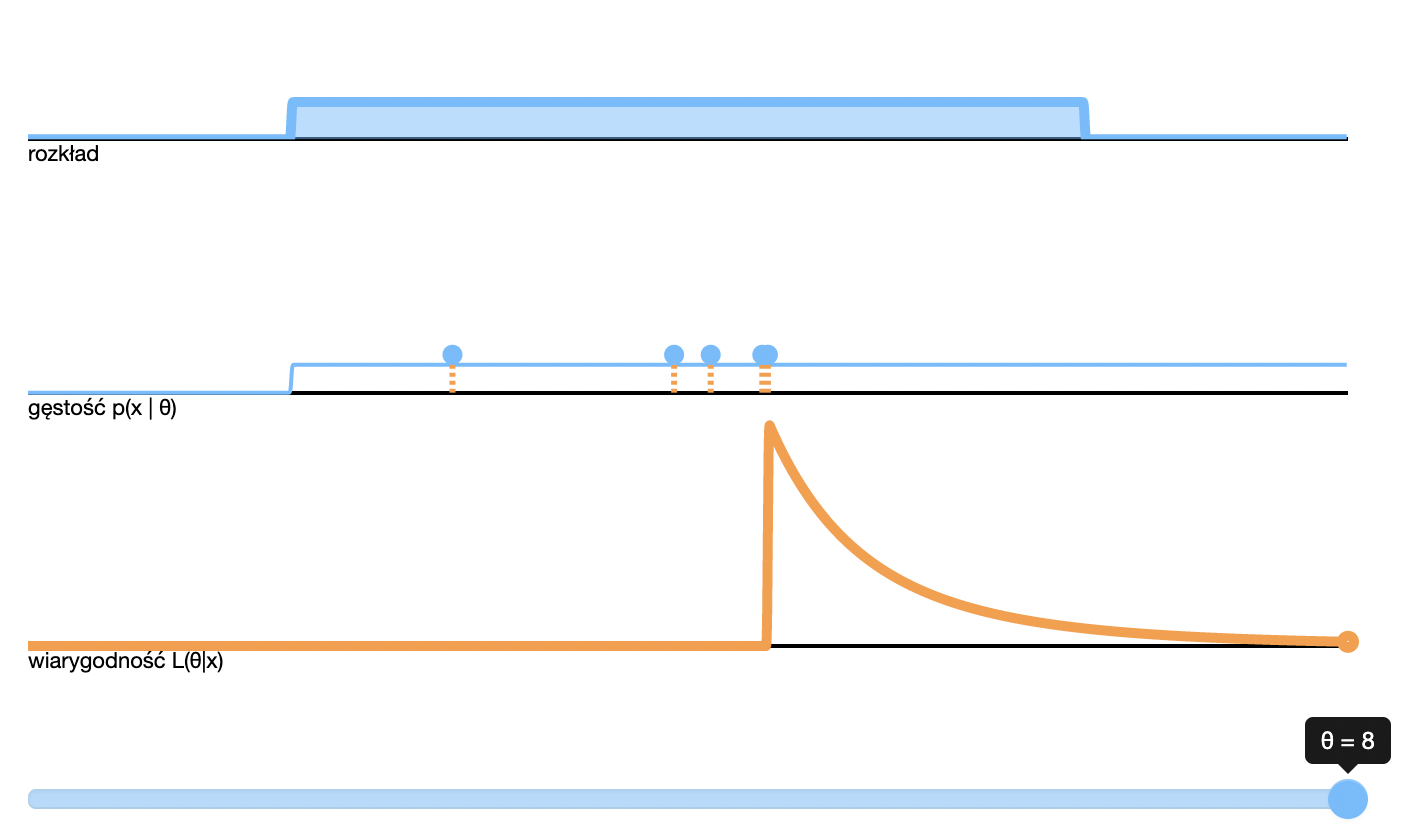
\includegraphics[scale=0.27]{images/likelihood-uniform}
        \caption{Rozkład jednostajny $(0, \theta)$ (rozmiar próbki - 5).}
    \end{minipage}
    \begin{minipage}{0.45\textwidth}
        \centering
        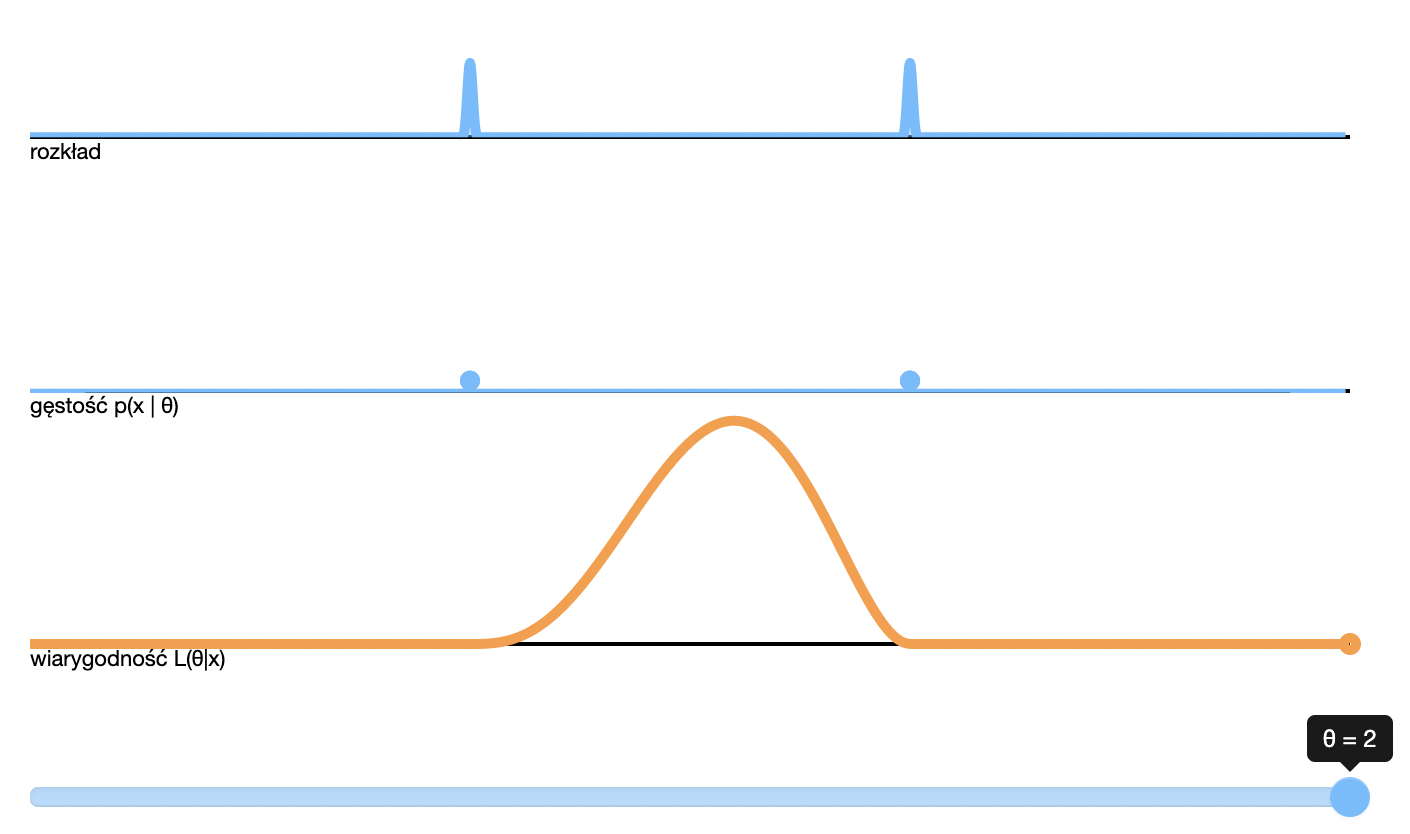
\includegraphics[scale=0.27]{images/likelihood-zero-one}
        \caption{Rozkład zero jedynkowy $(0, \theta)$ (rozmiar próbki - 5).}
    \end{minipage}
\end{figure}

\begin{align*}
    \text{Twierdzenie Bayesa: } & & P(A|B)=\frac{P(B|A) P(A)}{P(B)} \\
    \text{Funkcja wiarygodności: } & & L(\theta|x)=P(x|\theta) \\
    \text{Iloraz wiarygodności: } & & \Lambda(\theta_1 : \theta_2 | x)=\frac{L(\theta_1 | x)}{L(\theta_2 | x)}
\end{align*}

W statystyce bayesowskiej \textbf{zasada niezmienniczości ilorazu funkcji wiarygodności} nie zachodzi.
Przekształcenia (tranformacja) parametru zmienia iloraz.